\documentclass[11pt, handout]{beamer}

% Allgemeine Definitionen
\usepackage[english]{babel}	% Deutsche Sprachanpassung, z.B. Silbentrennung bei Worten mit Sonderzeichen
\usepackage[utf8]{inputenc}		% Direkte Eingabe von Umlauten

\usepackage{multimedia}		% Animations-Unterstützung (braucht hyperref | hyperref ist Teil von beamer )
\usepackage{xcolor}
\usepackage{fancyvrb}


% Verschiedene Operatoren
\newcommand{\union}{\ensuremath{\cup}}		% Die Vereinigung
\newcommand{\schnitt}{\ensuremath{\cap}}		% Der Schnitt
\newcommand{\und}{\ensuremath{\wedge}}		% Das und-Symbol
\newcommand{\oder}{\ensuremath{\vee}}		% Das oder-Symbol
\newcommand{\folgt}[1]{\ensuremath{\stackrel{#1}{\Rightarrow}}}	% Das Folgerungszeichen mit Symbol darüber 
\newcommand{\gleich}[1]{\ensuremath{\stackrel{#1}{=}}}	% Das Gleichheitszeichen mit Symbol darüber 
\newcommand{\isdef}{\ensuremath{\mathrel{\mathop:}=}}		% Das "ist-definiert"-Zeichen
\newcommand{\defis}{\ensuremath{=\mathrel{\mathop:}}}		% Das "ist-definiert"-Zeichen (andersrum)

% Weiterer nützlicher Kram
%\usepackage{enumitem}		% NICHT kompatibel mit beamer!
\usepackage{amsfonts, amsmath, amssymb}
\usepackage{amsthm}			% Eigene Umgebungen
\usepackage{thumbpdf}	% Seitenvorschau in PDF-Dokumenten

\usepackage{nicefrac}

\usepackage{pgf, tikz}
\usetikzlibrary{arrows, decorations.pathreplacing, calc, decorations.pathmorphing, shapes}

% Erst die Farbe (optional), dann die Norm, dann der Inhalt
\newcommand{\norm}[3][black]{\ensuremath{\left\Vert #3\right\Vert_{\textcolor{#1}{#2}}}}

% Die folgenden Befehle dienen dazu, verschiedene Konventionen darzustellen. Man kann damit
% auf einfache Weise die in dem Dokument verwendeten Konventionen umschalten.

%\newcommand{\bisn}[1]{\ensuremath{\underline{#1}}}	% Bezeichnung für die Menge {1,..,n}
\newcommand{\bisn}[1]{\ensuremath{\{1,\dots , #1 \}}}	% Alternative (ohne Fallunterscheidung)

% Das Erzeugnis, das erste Argument zeigt an, welches Erzeugnis gemeint ist, das zweite gibt seinen Inhalt an.
%\newcommand{\spn}[2][]{\ensuremath{\mathrm{span} \{ #1 \}}}
\newcommand{\spn}[2][]{\ensuremath{\left\langle #2 \right\rangle _{ #1 }}}

\newcommand{\grad}[1]{\ensuremath{\mathrm{grad}( #1 )}}
%\newcommand{\grad}[1]{\ensuremath{\nabla #1}}

\newcommand{\tr}[1]{\ensuremath{#1^{tr}}} % Bezeichnung für die Transponierte einer Matrix

% Die Mengentheoretische Differenz
\newcommand{\ohne}{\ensuremath{-}}
%\newcommand{\ohne}{\ensuremath{\backslash}}

\DeclareMathOperator{\Hom}{Hom}
\DeclareMathOperator{\GL}{GL}
\DeclareMathOperator{\diag}{diag}
\DeclareMathOperator{\Rg}{Rang}
\DeclareMathOperator{\Bild}{Bild}
\DeclareMathOperator{\Kern}{Kern}
\DeclareMathOperator{\Spur}{Spur}
\DeclareMathOperator{\Aut}{Aut}
\DeclareMathOperator{\Sym}{Sym}
\DeclareMathOperator{\Pot}{Pot}
\DeclareMathOperator{\Grad}{Grad}
\DeclareMathOperator{\kgV}{kgV}

\newcommand{\menge}[1]{\ensuremath{\mathbb{#1}}}
\newcommand{\N}{\menge{N}}
\newcommand{\Z}{\menge{Z}}
\newcommand{\Q}{\menge{Q}}
\newcommand{\R}{\menge{R}}
\newcommand{\C}{\menge{C}}

% Mit den schönen Buchstaben arbeiten
\renewcommand{\phi}{\varphi}

\renewcommand{\subset}{\subseteq}

% Verschiedene mögliche Umgebungen
\newtheorem{lem}{Lemma}[section]		% Lemma
\newtheorem{bsp}[lem]{Beispiel}		% Beispiel
\newtheorem{folg}[lem]{Folgerung}	% Folgerung
\newtheorem{bem}[lem]{Bemerkung}
\newtheorem{satz}[lem]{Satz}			% Satz
\newtheorem{kor}[lem]{Korollar}		% Korollar
%\newtheorem{alg}[lem]{Algorithmus}	% Algorithmus
%\theoremstyle{definition}
\newtheorem{defi}[lem]{Definition}	% Definition
\theoremstyle{remark}
\newtheorem*{idea}{Beweisidee}	% Beweisidee (vor dem eigentlichen Beweis)




\beamertemplatenavigationsymbolsempty

\usetheme{Boadilla}
%	AnnArbor | Antibes | Bergen |
%	Berkeley | Berlin | Boadilla |
%	boxes | CambridgeUS | Copenhagen |
%	Darmstadt | default | Dresden |
%	Frankfurt | Goettingen |Hannover |
%	Ilmenau | JuanLesPins | Luebeck |
%	Madrid | Malmoe | Marburg |
%	Montpellier | PaloAlto | Pittsburgh |
%	Rochester | Singapore | Szeged |
%	Warsaw
%\usecolortheme{seahorse}
%	albatross | beaver | beetle |
%	crane | default | dolphin |
%	dove | fly | lily | orchid |
%	rose |seagull | seahorse |
%	sidebartab | structure |
%	whale | wolverine
%\usefonttheme{professionalfonts}
%	default | professionalfonts | serif |
%	structurebold | structureitalicserif |
%	structuresmallcapsserif
%\useinnertheme{rounded}
%	circles | default | inmargin |
%	rectangles | rounded
%\useoutertheme{shadow}
%	default | infolines | miniframes |
%	shadow | sidebar | smoothbars |
%	smoothtree | split | tree

% Graphic support
% This document contains the TikZ-header for all our LaTeX-computations.
% It especially contains all global graphic parameters.

\usepackage{amsmath, amssymb, amsfonts} % Standard Math-stuff

\usepackage{tikz}
\usetikzlibrary{calc}
\usetikzlibrary{positioning}

% Define a text=none option for nodes that ignores the given text, from
% https://tex.stackexchange.com/questions/59354/no-text-none-in-tikz
\makeatletter
\newif\iftikz@node@phantom
\tikzset{
  phantom/.is if=tikz@node@phantom,
  text/.code=%
    \edef\tikz@temp{#1}%
    \ifx\tikz@temp\tikz@nonetext
      \tikz@node@phantomtrue
    \else
      \tikz@node@phantomfalse
      \let\tikz@textcolor\tikz@temp
    \fi
}
\usepackage{etoolbox}
\patchcmd\tikz@fig@continue{\tikz@node@transformations}{%
  \iftikz@node@phantom
    \setbox\pgfnodeparttextbox\hbox{}
  \fi\tikz@node@transformations}{}{}
\makeatother

% Now we define the global styles
% The global styles are defined nestedly. You have to give your tikzpicture
% the global options [vertexStyle, edgeStyle, faceStyle] to activate them.
% 
% You can disable labels by using the option nolabels, i.e. 
% vertexStyle=nolabels to deactivate vertex labels.
%
% If you want to have a specific style for your picture, you can also use
% this specific meta-style instead of the general style. For example if you
% want to use double edges in one single picture - no matter the style of
% the rest of the document - you can use edgeDouble instead of edgeStyle.
%
% To set the default style, modify the vertexStyle/.default entry.

% Vertex styles
\tikzset{ 
    vertexNodePlain/.style = {fill=gray, shape=circle, inner sep=0pt, minimum size=2pt, text=none},
    vertexPlain/labels/.style = {
        vertexNode/.style={vertexNodePlain},
        vertexLabel/.style={gray}
    },
    vertexPlain/nolabels/.style = {
        vertexNode/.style={vertexNodePlain},
        vertexLabel/.style={text=none}
    },
    vertexPlain/.style = vertexPlain/#1,
    vertexPlain/.default=labels
}
\tikzset{
    vertexNodeNormal/.style = {fill=blue, shape=circle, inner sep=0pt, minimum size=4pt, text=none},
    vertexNormal/labels/.style = {
        vertexNode/.style={vertexNodeNormal},
        vertexLabel/.style={blue}
    },
    vertexNormal/nolabels/.style = {
        vertexNode/.style={vertexNodeNormal},
        vertexLabel/.style={text=none}
    },
    vertexNormal/.style = vertexNormal/#1,
    vertexNormal/.default=labels
}
\tikzset{
    vertexNodeBall/.style = {shape=circle, ball color=orange, inner sep=2pt, outer sep=0pt, minimum size=3pt},
    vertexBall/labels/.style = {
        vertexNode/.style={vertexNodeBall, text=black},
        vertexLabel/.style={text=none}
    },
    vertexBall/nolabels/.style = {
        vertexNode/.style={vertexNodeBall, text=none},
        vertexLabel/.style={text=none}
    },
    vertexBall/.style = vertexBall/#1,
    vertexBall/.default=labels
}
\tikzset{ 
    vertexStyle/.style={vertexNormal=#1},
    vertexStyle/.default = labels
}


% 1) position of the vertex
% 2) relative position of the node
% 3) name of the vertex
\newcommand{\vertexLabelR}[3]{
    \node[vertexLabel, #2] at (#1) {#3};
}
% 1) position of the vertex
% 2) absolute position of the node
% 3) name of the vertex
\newcommand{\vertexLabelA}[3]{
    \node[vertexLabel] at (#2) {#3};
}


% Edge styles
% If you have trouble with the double-lines overlapping, this might (?) help:
% https://tex.stackexchange.com/questions/288159/closing-the-ends-of-double-line-in-tikz
\tikzset{
    edgeLinePlain/.style={line join=round},
    edgePlain/labels/.style = {
        edge/.style={edgeLinePlain},
        edgeLabel/.style={fill=blue!20!white}
    },
    edgePlain/nolabels/.style = {
        edge/.style={edgeLinePlain},
        edgeLabel/.style={text=none}
    },
    edgePlain/.style = edgePlain/#1,
    edgePlain/.default = labels
}
\tikzset{
    edgeLineDouble/.style = {thin, double=gray!90!white, double distance=.3pt, line join=round},
    edgeDouble/labels/.style = {
        edge/.style = {edgeLineDouble},
        edgeLabel/.style = {fill=blue!20!white}
    },
    edgeDouble/nolabels/.style = {
        edge/.style = {edgeLineDouble},
        edgeLabel/.style = {text=none}
    },
    edgeDouble/.style = edgeDouble/#1,
    edgeDouble/.default = labels
}
\tikzset{
    edgeStyle/.style = {edgePlain=#1},
    edgeStyle/.default = labels
}

% Face styles
% Here we have an exception - the style face is always defined.
% 
\newcommand{\faceColorY}{yellow!60!white}   % yellow
\newcommand{\faceColorB}{blue!60!white}     % blue
\newcommand{\faceColorP}{cyan!60}           % purple
\newcommand{\faceColorR}{red!60!white}      % red
\newcommand{\faceColorG}{green!60!white}    % green
\newcommand{\faceColorO}{orange!50!yellow!70!white} % orange

\newcommand{\faceColor}{\faceColorY}
\newcommand{\faceColorSwap}{\faceColorB}
\tikzset{
    face/.style = {fill=#1},
    face/.default = \faceColor,
    faceY/.style = {face=\faceColorY},
    faceB/.style = {face=\faceColorB},
    faceP/.style = {face=\faceColorP},
    faceR/.style = {face=\faceColorR},
    faceG/.style = {face=\faceColorG},
    faceO/.style = {face=\faceColorO}
}
\tikzset{
    faceStyle/labels/.style = {
        faceNode/.style = {}
    },
    faceStyle/nolabels/.style = {
        faceNode/.style = {text=none}
    },
    faceStyle/.style = faceStyle/#1,
    faceStyle/.default = labels
}
\tikzset{ face/.style={fill=#1} }
\tikzset{ faceSwap/.code=
    \ifdefined\swapColours
        {face=\faceColorSwap}
    \else
        {face=\faceColor}
    \fi
}

% Sometimes we want to implement different behaviour for the generated 
% HTML-pictures (for example, shading is not supported in HTML).
% For that we define a macro to check whether we run the code with
% htlatex. The code comes from 
% https://tex.stackexchange.com/questions/93852/what-is-the-correct-way-to-check-for-latex-pdflatex-and-html-in-the-same-latex
\makeatletter
\edef\texforht{TT\noexpand\fi
  \@ifpackageloaded{tex4ht}
    {\noexpand\iftrue}
    {\noexpand\iffalse}}
\makeatother


\usepackage{hyperref}




\author{Markus Baumeister}
\title{Simplicial surfaces in GAP}
\date{??.08.2017}

\begin{document}

% Titelseite
\begin{frame}
\titlepage
\end{frame}


\begin{frame}
    \tableofcontents
\end{frame}


%%%%%%%%%%%%%%%%%%%%%%%%%%%%%%%%%%%%%%%%%%%%%%%%%%%
%%
%%    First section
%%
\section{General simplicial surfaces}
\frame{\tableofcontents[currentsection]}

\begin{frame}{\uncover<3->{Triangular complexes}}
    We want to describe different structures:
    \uncover<2->{
        \begin{center}
            \begin{tikzpicture}[scale=2]
    \begin{scope}[scale=0.5,yshift=0.8cm]
                    % Coordinates of octahedron
                \def\len{2} % The length of the base
                \def\h{0.9}   % \h*\len is the hight of the apex above the 
                            % center of the square
                \coordinate (Mid) at (0,0);
                \coordinate (Right) at (0.5*\len,0.3*\len);
                \coordinate (Left) at (-0.75*\len,0.25*\len);
                \coordinate (Back) at ($(Right)+(Left)$);
                \coordinate (Center) at ($(Left)!0.5!(Right)$);
                \coordinate (Up) at ($(Center)+(0,\h*\len)$);
                \coordinate (Down) at ($(Center)+(0,-\h*\len)$);

                \filldraw[face] (Up) -- (Mid) -- (Left) -- cycle;
                \filldraw[face] (Up) -- (Mid) -- (Right) -- cycle;
                \filldraw[face] (Down) -- (Mid) -- (Left) -- cycle;
                \filldraw[face] (Down) -- (Mid) -- (Right) -- cycle;
                \draw[dashed] (Up) -- (Back) -- (Down);
                \draw[dashed] (Left) -- (Back) -- (Right);

 

    \end{scope}
    
    \begin{scope}[xshift=1cm]
        			    \coordinate (A) at (0,0);
			    \coordinate (B) at (1.7,0.5);
			    \coordinate (C) at (1.3,1.4);
			    \coordinate (D) at (0.5,1.5);
			    \coordinate (E) at (1,0.7);
			
			    % Take care to draw the faces in the back first
                            \draw[face,edge]
                                (A) -- (B) -- (C) -- cycle
                                (A) -- (C) -- (D) -- cycle;
                            \draw[face,edge]
                                (A) -- (B) -- (E) -- cycle
                                (A) -- (E) -- (D) -- cycle;
                            \draw[edge, dashed] (A) -- (C);

    \end{scope}

    \begin{scope}[xshift=3.5cm]
        			    \coordinate (A) at (0,0);
			    \coordinate (B) at (1.3,0.4);
			    \coordinate (C) at (0.4,1.3);
			
			    \filldraw[face] (A) -- (B) to[bend right=45] (C) -- cycle;
			    \filldraw[face] (A) -- (B) to[bend left=45] (C) -- cycle;


    \end{scope}
\end{tikzpicture}


        \end{center}
    }
    \uncover<3->{
        $\leadsto$ \textbf{triangular complexes}
    }
    \begin{itemize}
        \item<4-> sets of vertices, edges and faces
        \item<5-> incidence relation between them
        \item<6-> every face is a triangle
        \item<7-> every vertex lies in an edge \uncover<8->{and every edge lies in a face}
    \end{itemize}
\end{frame}


\begin{frame}{Isomorphism testing}
    Incidence structure can be interpreted as a coloured graph:
    \begin{center}
        \begin{tikzpicture}[vertexNode/.style={circle,fill=\colorVertexNode},node distance=0.5,
                faceNode/.style={fill=\faceColor,regular polygon, regular polygon sides=3}]
            \def\len{1.5}
            
            \uncover<4->{
                \coordinate[label={[vertex]left:5}] (A) at (0,0);
                \coordinate[label={[vertex]above:6}] (B) at (\len,\len);
                \coordinate[label={[vertex]below:7}] (C) at (\len,-\len);
            }
            \uncover<7->{
                \coordinate[label={[vertex]right:11}] (D) at (2*\len,0);
            }

            \uncover<2->{
                \filldraw[face] (A) -- (B) -- (C) -- cycle;
                \node at (barycentric cs:A=1,B=1,C=1) {1};
            }
            \uncover<5->{
                \filldraw[face] (B) -- (C) -- (D) -- cycle;
                \node at (barycentric cs:B=1,C=1,D=1) {8};
            }

            \uncover<3->{
                \drawEdge{A}{B}{2}
                \drawEdge{A}{C}{3}
                \drawEdge{B}{C}{4}
            }
            \uncover<6->{
                \drawEdge{B}{D}{9}
                \drawEdge{C}{D}{10}
            }

            \uncover<4->{
                \fill[vertex] (A) circle (\vSize);
                \fill[vertex] (B) circle (\vSize);
                \fill[vertex] (C) circle (\vSize);
            }
            \uncover<7->{
                \fill[vertex] (D) circle (\vSize);
            }


            \begin{scope}[xshift=5cm]
                \uncover<3->{
                    \node[edgeBackground] (E1) {2};
                    \node[edgeBackground] (E2) [right=of E1] {3};
                    \node[edgeBackground] (E3) [right=of E2] {4};
                }
                \uncover<6->{
                    \node[edgeBackground] (E4) [right=of E3] {9};
                    \node[edgeBackground] (E5) [right=of E4] {10};
                }

                \uncover<2->{
                    \node[faceNode] (F1) [above=of E2] {1}; 
                }
                \uncover<5->{
                    \node[faceNode] (F2) [above=of E4] {8};
                }

                \uncover<4->{
                    \node[vertexNode] (V1) [below=of E1] {5}
                        edge (E1) edge (E2);
                    \node[vertexNode] (V2) [right=of V1] {6}
                        edge (E1) edge (E3);
                    \node[vertexNode] (V3) [right=of V2] {7}
                        edge (E2) edge (E3);
                }
                \uncover<7->{
                    \node[vertexNode] (V4) [right=of V3] {11}
                        edge (E4) edge (E5);
                }

                \uncover<3->{
                    \draw (F1) -- (E1);
                    \draw (F1) -- (E2);
                    \draw (F1) -- (E3);
                }

                \uncover<5->{
                    \draw (F2) -- (E3);
                }

                \uncover<6->{
                    \draw (F2) -- (E4) -- (V2);
                    \draw (F2) -- (E5) -- (V3);
                }
            \end{scope}
        \end{tikzpicture}
    \end{center}

    \uncover<8->{
        $\leadsto$ reduce to graph isomorphism problem
    }

    \uncover<9->{
        $\leadsto$ can be solved quite easily by \texttt{Nauty} (McKay, Piperno)
    }

    \uncover<10->{
        Interfaced by NautyTracesInterface (by Gutsche, Niemeyer, Schweitzer)
        \begin{itemize}
            \item<11-> direct C--interface without writing files
            \item<12-> also returns automorphism group
        \end{itemize}
    }
\end{frame}


\begin{frame}{General properties}
    \pause
    Some properties can be computed for all triangular complexes:
    \pause
    \begin{itemize}
        \item Connectivity
        \pause
        \item Euler--Characteristic
    \end{itemize}
    \pause
    \textit{Orientability} is \textbf{not} one of them.
    \pause
    Counterexample:
        \begin{center}
            \begin{tikzpicture}
                \coordinate (A) at (0,0);
\coordinate (B) at (0,1.5);
\coordinate (C) at (-0.7,0.4);
\coordinate (D) at (0.8,0.4);
\coordinate (E) at (0.9,0.8);
			
\draw[edge, face]
    (A) -- (B) -- (E) -- cycle;
\draw[edge,face]
    (A) -- (B) -- (C) -- cycle
    (A) -- (B) -- (D) -- cycle;
\draw[edge, dashed] (A) -- (E);
		     

	    \end{tikzpicture}
        \end{center}
    \pause
    $\Rightarrow$ every edge lies in at most two faces (for well--definedness)
    
    \pause
    $\leadsto$ \textbf{ramified simplicial surfaces}
\end{frame}


\begin{frame}{Why ramified?}
    \pause
    Typical example of ramified simplicial surface:
    \pause
    \begin{center}
        \begin{tikzpicture}
            \begin{tikzpicture}[vertexBall, edgeDouble, faceStyle, scale=2]

% Define the coordinates of the vertices
\coordinate (V1_1) at (0., 0.);
\coordinate (V2_1) at (1., 0.);
\coordinate (V3_1) at (-0.5, 0.8660254037844384);
\coordinate (V3_2) at (1.5, 0.8660254037844388);
\coordinate (V4_1) at (0.4999999999999999, 0.8660254037844386);
\coordinate (V5_1) at (0.5000000000000001, -0.8660254037844386);
\coordinate (V5_2) at (-0.9999999999999996, 0.);
\coordinate (V5_3) at (2., 0.);


% Fill in the faces
\fill[face]  (V2_1) -- (V4_1) -- (V1_1) -- cycle;
\node[faceLabel] at (barycentric cs:V2_1=1,V4_1=1,V1_1=1) {$1$};
\fill[face]  (V2_1) -- (V3_2) -- (V4_1) -- cycle;
\node[faceLabel] at (barycentric cs:V2_1=1,V3_2=1,V4_1=1) {$2$};
\fill[face]  (V4_1) -- (V3_1) -- (V1_1) -- cycle;
\node[faceLabel] at (barycentric cs:V4_1=1,V3_1=1,V1_1=1) {$3$};
\fill[face]  (V1_1) -- (V5_1) -- (V2_1) -- cycle;
\node[faceLabel] at (barycentric cs:V1_1=1,V5_1=1,V2_1=1) {$4$};
\fill[face]  (V3_1) -- (V5_2) -- (V1_1) -- cycle;
\node[faceLabel] at (barycentric cs:V3_1=1,V5_2=1,V1_1=1) {$5$};
\fill[face]  (V2_1) -- (V5_3) -- (V3_2) -- cycle;
\node[faceLabel] at (barycentric cs:V2_1=1,V5_3=1,V3_2=1) {$6$};


% Draw the edges
\draw[edge] (V2_1) -- node[edgeLabel] {$1$} (V1_1);
\draw[edge] (V1_1) -- node[edgeLabel] {$2$} (V3_1);
\draw[edge] (V1_1) -- node[edgeLabel] {$3$} (V4_1);
\draw[edge] (V5_1) -- node[edgeLabel] {$4$} (V1_1);
\draw[edge] (V1_1) -- node[edgeLabel] {$4$} (V5_2);
\draw[edge] (V3_2) -- node[edgeLabel] {$5$} (V2_1);
\draw[edge] (V4_1) -- node[edgeLabel] {$6$} (V2_1);
\draw[edge] (V2_1) -- node[edgeLabel] {$7$} (V5_1);
\draw[edge] (V5_3) -- node[edgeLabel] {$7$} (V2_1);
\draw[edge] (V3_1) -- node[edgeLabel] {$8$} (V4_1);
\draw[edge] (V4_1) -- node[edgeLabel] {$8$} (V3_2);
\draw[edge] (V5_2) -- node[edgeLabel] {$9$} (V3_1);
\draw[edge] (V3_2) -- node[edgeLabel] {$9$} (V5_3);


% Draw the vertices
\vertexLabelR{V1_1}{left}{$1$}
\vertexLabelR{V2_1}{left}{$2$}
\vertexLabelR{V3_1}{left}{$3$}
\vertexLabelR{V3_2}{left}{$3$}
\vertexLabelR{V4_1}{left}{$4$}
\vertexLabelR{V5_1}{left}{$5$}
\vertexLabelR{V5_2}{left}{$5$}
\vertexLabelR{V5_3}{left}{$5$}

\end{tikzpicture}

        \end{tikzpicture}
    \end{center}
    \pause
    $\Rightarrow$ It is not a surface -- there is a \textit{ramification} at 
        the central vertex
    
    \pause
    A \textbf{simplicial surface} does not have these ramifications.
\end{frame}


\begin{frame}{Classification}
    \pause
    Plesken/Strzelczyk classified all closed simplicial surfaces up to 20 triangles.

    \begin{itemize}
        \pause
        \item only interesting for those without a 3--cycle of edges
        \pause
        \item e.\,g. there are 87 non--isomorphic surfaces with 20 triangles
        \pause
        \item e.\,g. there is only one surface with 10 triangles:
    \end{itemize}

    \pause
    \begin{center}
        \begin{tikzpicture}
            TODO
        \end{tikzpicture}
    \end{center}
\end{frame}


\begin{frame}{Progress report of simplicial surfaces}
    \pause
    Already implemented:
    \begin{itemize}
        \pause
        \item surface hierarchy
        \pause
        \item elementary properties (e.\,g. connectivity, orientability)
        \pause
        \item isomorphism testing
        \pause
        \item classification data base of small surfaces
    \end{itemize}

    \pause
    Not yet implemented:
    \begin{itemize}
        \pause
        \item automorphism group
        \pause
        \item advanced properties (any wishes?)
    \end{itemize}
\end{frame}

            
%%%%%%%%%%%%%%%%%%%%%%%%%%%%%%%%%%%%%%%%%%%%%%%%%%%%%%%%%%
%%
%%              Second section
%%
\section{Edge colouring and group properties}
\newcommand{\colA}{blue}
\newcommand{\colB}{red}
\newcommand{\colC}{green!80!black}
\newcommand{\width}{very thick}
\frame{\tableofcontents[currentsection]}


\begin{frame}{Embedding question}
    \pause
    Given: A polygonal complex
    \begin{itemize}
        \pause
        \item Can it be embedded?
        \pause
        \item In how many ways?
    \end{itemize}
    \pause
    Simplifications:
    \begin{enumerate}
        \pause
        \item Only polygonal surfaces (surface that is build from polygons)
        \pause
        \item All polygons are triangles (\textbf{simplicial surfaces})
        \pause
        \item All triangles are isometric
    \end{enumerate}
    \pause
    $\leadsto$ Edge--colouring encodes different lengths
            \begin{center}
                %       F
                %    C     E 
                % A     B    D
                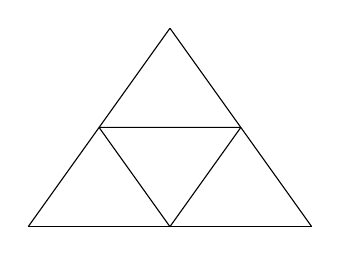
\begin{tikzpicture}[scale=0.9]
                    \coordinate (A) at (0,0);
                    \coordinate (B) at (2,0);
                    \coordinate (C) at (1,1.4);
                    \coordinate (D) at ($2*(B)$);
                    \coordinate (E) at ($(B)+(C)$);
                    \coordinate (F) at ($2*(C)$);

                    \draw[\colA, \width] (A) -- (B) -- (D);
                    \draw[\colA, \width] (C) -- (E);
                    \draw[\colB, \width] (B) -- (C);
                    \draw[\colB, \width] (D) -- (E) -- (F);
                    \draw[\colC, \width] (A) -- (C) -- (F);
                    \draw[\colC, \width] (B) -- (E);
                \end{tikzpicture}
            \end{center}
\end{frame}


\begin{frame}{Colouring as permutation}
    \onslide<2->{
        Consider tetrahedron \onslide<4->{with edge colouring}
    }

    \begin{center}
        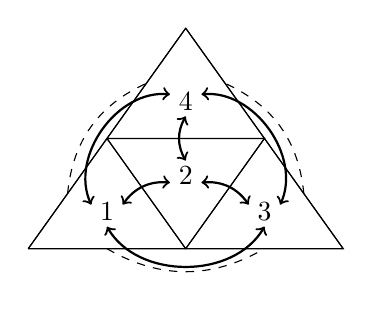
\begin{tikzpicture}
                \coordinate (A) at (0,0);
                \coordinate (B) at (2,0);
                \coordinate (C) at (1,1.4);
                \coordinate (D) at ($2*(B)$);
                \coordinate (E) at ($(B)+(C)$);
                \coordinate (F) at ($2*(C)$);
            \onslide<3->{
                \draw (A) -- (B) -- (D) -- (E) -- (F) -- (C) -- (E) -- (B) -- (C) -- (A);
                \node at (barycentric cs:A=1,B=1,C=1) {1};
                \node at (barycentric cs:B=1,C=1,E=1) {2};
                \node at (barycentric cs:B=1,D=1,E=1) {3};
                \node at (barycentric cs:C=1,E=1,F=1) {4};
                \draw[dashed] ($(A)!0.5!(C)$) to[bend left] ($(C)!0.5!(F)$);
                \draw[dashed] ($(A)!0.5!(B)$) to[bend right] ($(B)!0.5!(D)$);
                \draw[dashed] ($(D)!0.5!(E)$) to[bend right] ($(E)!0.5!(F)$);
            }
            \onslide<5->{
                \draw[\colA, \width] (A) -- (B) -- (D);
                \draw[\colA, \width] (C) -- (E);
                \draw[\colB, \width] (B) -- (C);
                \draw[\colB, \width] (D) -- (E) -- (F);
                \draw[\colC, \width] (A) -- (C) -- (F);
                \draw[\colC, \width] (B) -- (E);
            }

            % Draw switching arrows
            \onslide<9-11>{
                \draw[<->,\colB, thick] (barycentric cs:A=1,B=2,C=2) to[bend left] (barycentric cs:B=2,C=2,E=1);
            }
            \onslide<10-11>{
                \draw[<->,\colB,thick] (barycentric cs:B=1,D=2,E=2) to[bend right=60] (barycentric cs:E=2,F=2,C=1);
            }
            \onslide<12>{
                \draw[<->,\colA,thick] (barycentric cs:A=2,B=2,C=1) to[bend right=60] (barycentric cs:B=2,D=2,E=1);
                \draw[<->,\colA,thick] (barycentric cs:C=2,E=2,B=1) to[bend left] (barycentric cs:C=2,E=2,F=1);
            }
            \onslide<13>{
                \draw[<->,\colC,thick] (barycentric cs:A=2,B=1,C=2) to[bend left=60] (barycentric cs:C=2,E=1,F=2);
                \draw[<->,\colC,thick] (barycentric cs:B=2,C=1,E=2) to[bend left] (barycentric cs:B=2,D=1,E=2);
            }
        \end{tikzpicture}
    \end{center}
    \onslide<6->{
        \textit{simplicial surface} $\Rightarrow$ \onslide<7->{at most two faces at each edge}
    
        \onslide<8->{
            $\leadsto$ every edge defines transposition of incident faces
        }

        \onslide<11->{
            $\leadsto$ every colour class defines permutation of the faces
        }

        \onslide<9->{\textcolor{\colB}{(1,2)}}\onslide<10->{\textcolor{\colB}{(3,4)}}
        \onslide<12->{, \textcolor{\colA}{(1,3)(2,4)}}
        \onslide<13->{, \textcolor{\colC}{(1,4)(2,3)}}

        \onslide<14->{
            $\leadsto$ group theoretic considerations
        }
    }


\end{frame}
         

\begin{frame}{How do faces fit together?}
    \onslide<2->{
        Consider a face of the surface \onslide<4->{and a neighbouring face}
    }

    \onslide<6->{
        The neighbour can be coloured in two ways:
    }
    \onslide<1->{
        \begin{center}
        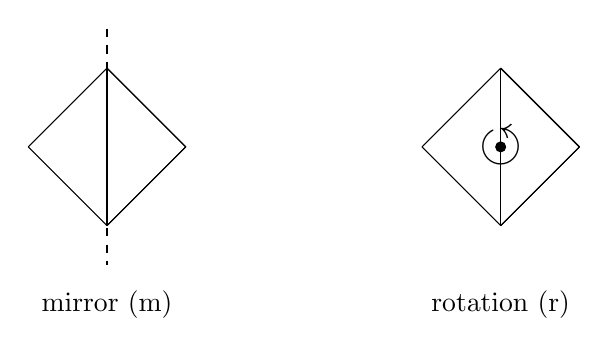
\begin{tikzpicture}
            % Numbers to determine drawing
            \def\x{1}
            \def\y{1}

            %      B
            %    / | \
            %   A  |  D
            %    \ | /
            %      C
            
            % First pair
            \begin{scope}
                \coordinate (A) at (0,0);
                \coordinate (B) at (\x,\y);
                \coordinate (C) at (\x,-\y);
                \coordinate (D) at (2*\x,0);

                \onslide<3->{
                    \draw[\colA,\width] (A) -- (B);
                    \draw[\colB,\width] (A) -- (C);
                    \draw[\colC,\width] (B) -- (C);
                }
                \onslide<5->{
                    \draw (B) -- (D) -- (C);
                }
                \onslide<7->{
                    \draw[\colA,\width] (B) -- (D);
                    \draw[\colB,\width] (C) -- (D);
                }
                \onslide<9->{
                    % Draw mirror line
                    \draw[dashed, thick] (\x,1.5*\y) -- (\x,-1.5*\y);
                    \node at (\x,-2*\y) {mirror (m)};
                }
            \end{scope}

            % Second pair
            \begin{scope}[xshift=5cm]
                \coordinate (A) at (0,0);
                \coordinate (B) at (\x,\y);
                \coordinate (C) at (\x,-\y);
                \coordinate (D) at (2*\x,0);

                \onslide<6->{
                    \draw[\colA,\width] (A) -- (B);
                    \draw[\colB,\width] (A) -- (C);
                    \draw[\colC,\width] (B) -- (C);
                    \draw (B) -- (D) -- (C);
                }
                \onslide<8->{
                    \draw[\colB,\width] (B) -- (D);
                    \draw[\colA,\width] (C) -- (D);
                }
                \onslide<10->{
                    % Draw rotation center and circle
                    \fill[black] (\x,0) circle (2pt);
                    \node[scale=2] at (\x,0) {$\circlearrowleft$};
                    \node at (\x,-2*\y) {rotation (r)};
                }
            \end{scope}
        \end{tikzpicture}
        \end{center}
    }
    \onslide<11->{
        This gives an \textbf{mr--assignment} for the edges.
    }

    \onslide<12->{
        Permutations and mr--assignment uniquely determine the surface.
    }
\end{frame}


\begin{frame}{Constructing surfaces from groups}
    \pause
    A general mr--assignment leads to complicated surfaces.
    
    \pause
    Simplification: edges of same colour have the same type

    \pause
    Example
        \begin{center}
            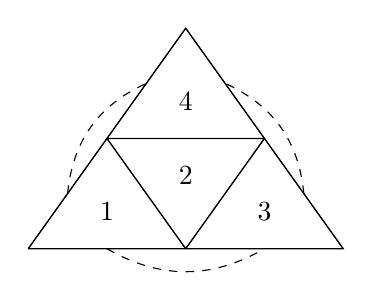
\begin{tikzpicture}
                \coordinate (A) at (0,0);
                \coordinate (B) at (2,0);
                \coordinate (C) at (1,1.4);
                \coordinate (D) at ($2*(B)$);
                \coordinate (E) at ($(B)+(C)$);
                \coordinate (F) at ($2*(C)$);

                \draw (A) -- (B) -- (D) -- (E) -- (F) -- (C) -- (E) -- (B) -- (C) -- (A);
                \node at (barycentric cs:A=1,B=1,C=1) {1};
                \node at (barycentric cs:B=1,C=1,E=1) {2};
                \node at (barycentric cs:B=1,D=1,E=1) {3};
                \node at (barycentric cs:C=1,E=1,F=1) {4};
                
                \draw[dashed] ($(A)!0.5!(C)$) to[bend left] ($(C)!0.5!(F)$);
                \draw[dashed] ($(A)!0.5!(B)$) to[bend right] ($(B)!0.5!(D)$);
                \draw[dashed] ($(D)!0.5!(E)$) to[bend right] ($(E)!0.5!(F)$);

                \draw[\colA, \width] (A) -- (B) -- (D);
                \draw[\colA, \width] (C) -- (E);
                \draw[\colB, \width] (B) -- (C);
                \draw[\colB, \width] (D) -- (E) -- (F);
                \draw[\colC, \width] (A) -- (C) -- (F);
                \draw[\colC, \width] (B) -- (E);
            \end{tikzpicture}
        \end{center}
    \pause
    has an rrr--structure

    \pause
    The easiest structure is an mmm--structure.
\end{frame}



%%%%%%%%%%%%%%%%%%%%%%%%%%%%%%%%%%%%%%%%%%%%%%%%%%%%%%%%%%%%%%
%%
%%    Third section
%%
\section{Abstract folding}
\frame{\tableofcontents[currentsection]}


\end{document}
